% !TEX root = vorlage.tex

\section{Proof of Concept}
\label{section:poc}
Zum Start des Projekts wird zusammen mit den betreuenden Kollegen eine Roadmap entworfen.
Diese bietet eine grobe Übersicht über die Arbeitsschritte und soll gerade zu Beginn bei der Strukturierung helfen.\\

Hierfür wird eine Confluence Seite eingerichtet, auf welcher die groben Arbeitsschritte, sowie Diagramme und weitere Informationen hinterlegt werden.
Außerdem wird eine Unterseite mit erstellt, auf welcher der Austausch im wöchentlichen Projektmeeting dokumentiert wird.
Hier können Informationen festgehalten werden, sowie Aufgaben mit zeitlicher Begrenzung zugeteilt werden.\\

Alle diese Schritte sollen zu einem erfolgreicheren Informationsaustausch, sowie Projektverlauf beitragen.


\subsection{Roadmap}
\label{section:roadmap}

Die Arbeitsschritte sind in einem initialen Projektmeeting zusammen mit den Betreuern entstanden.
Dabei fand ein Brainstorming statt und alle gesammelten Ideen wurden aufgeschrieben.\\

Allerdings mussten diese nun noch in eine logische Reihenfolge gebracht und in Kategorien unterteilt werden.
Diese geordnete und strukturierte Roadmap wurde im Nachgang auf der Hauptseite im Confluence als "Tasks" hinterlegt.\\

Dort dient sie als Übersicht zum aktuellen Projektstatus und um nachverfolgen zu können, welche Tätigkeiten noch erledigt werden müssen.
So können eventuell benötigte Ressourcen, wie zum Beispiel Testrechner, frühzeitig identifiziert werden.\\

\begin{figure}[H]
	\centering	
	\fbox{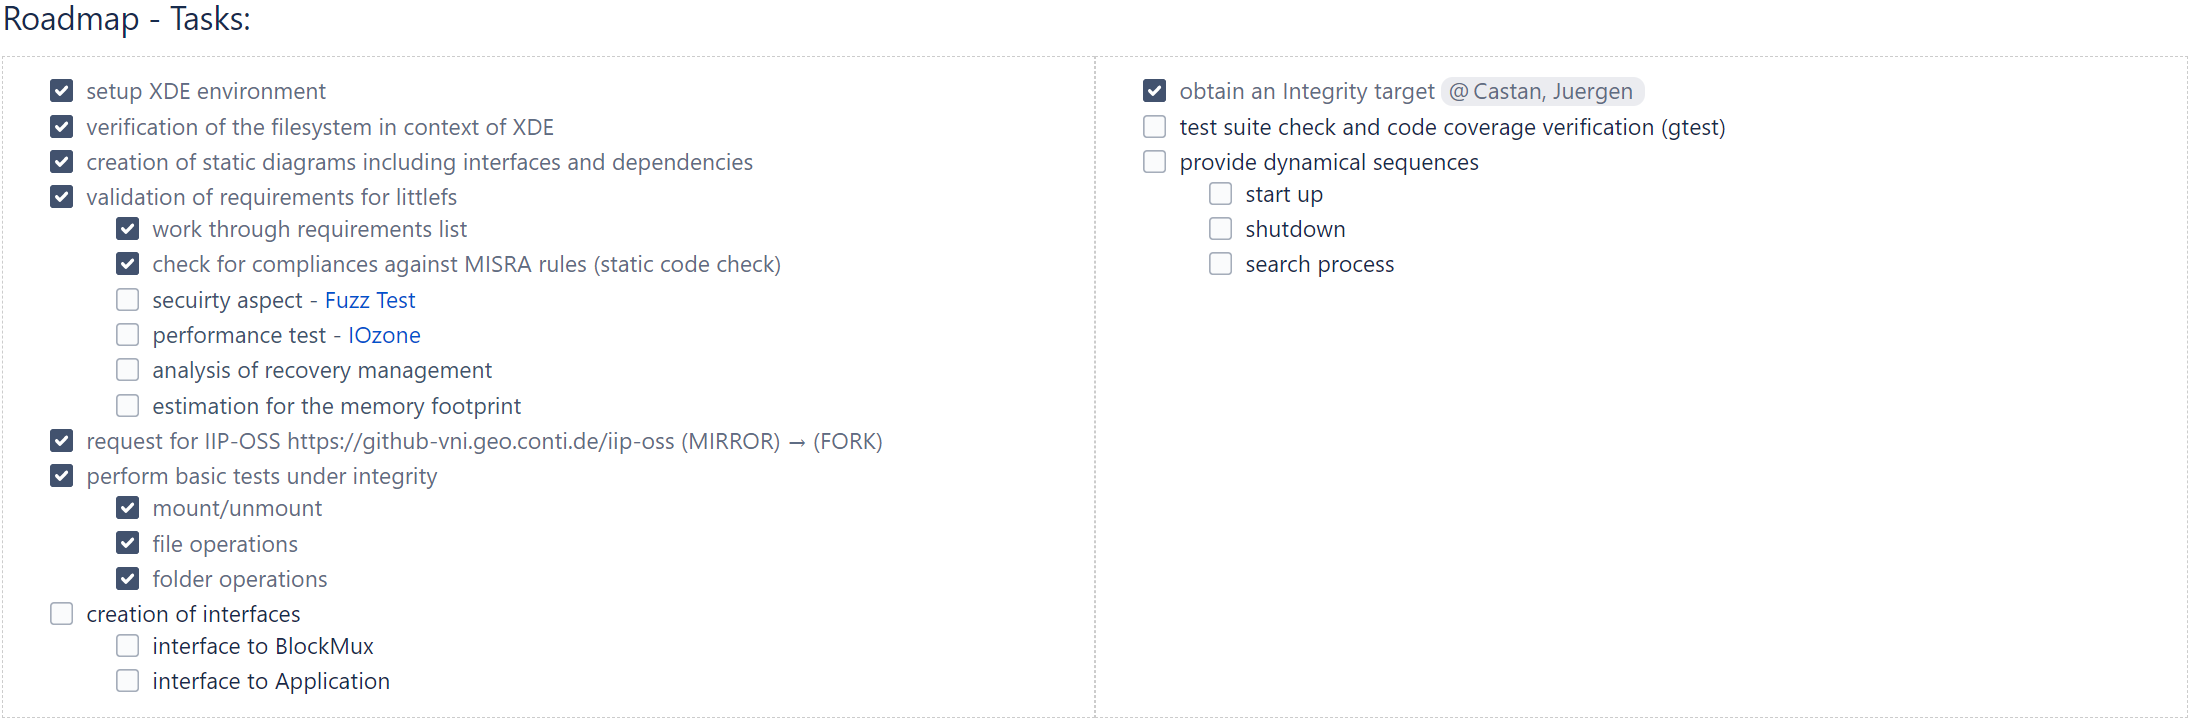
\includegraphics[width=1\textwidth]{Bilder/roadmap.png}}
	\caption{Roadmap}
	\label{fig:roadmap}
\end{figure}

Die Roadmap ist in zwei Bereiche aufgeteilt.
Auf der linken Seite ist ein chronologisch geplanter Ablauf von grob definierten Arbeitspaketen,
auf der rechten Seite hingegen Aufgaben welche nicht zum direkt Entwicklungsprozess zugehörig sind, jedoch trotzdem erledigt werden müssen.


\subsection{Einarbeitung}
\label{section:einarbeitung}
\textbf{?} Zu Beginn des Projekts war eine Einarbeitung in die nachfolgenden Themen unerlässlich.

\subsubsection{Dateisysteme}
Das Dateisystem ist verantwortlich für die Verwaltung von Daten auf einem Speichermedium und ist ein Teil des Betriebssystems.
Dabei kann sich die Art des \acl{DS}s je nach Speichermedium unterscheiden.
Ohne ein \acl{DS} wären die Daten im Speicher lediglich ein großer Datensatz und der Anfang, sowie Ende jedes Einzelnen wären nicht erkennbar.

Die Aufgabe des \acl{DS} ist es also die Daten zu schreiben, speichern, zu lesen und diese auch verändern zu können, sowie zu löschen.
Dabei definiert und spezifiziert das Dateisystem die Eigenschaften der Daten, so zum Beispiel:
\begin{itemize}
	\item Konvention für den Dateinamen
	\item Dateiattribute (erstellt, zuletzt bearbeitet, ...)
	\item Pfadlänge
\end{itemize}

Die \acl{DS}e unterscheiden sich  je nach Betriebssystem, da nicht jedes \acl{BS} jedes \acl{DS} unterstützt.
Nachfolgend eine Auflistung der gängigen \acl{DS} nach \acl{BS}.
\begin{itemize}
	\item Windows:	FAT, FAT16, FAT32, NTFS
	\item macOS:	HFS, HFS+
	\item Linux:	Ext2, Ext3, Ext3
\end{itemize}

% Charakteristiak der Dateisysteme?


\subsubsection{littlefs}
"A little fail-safe filesystem" oder auch littlefs ist ein aus der embedded Welt stammendes \acl{DS}.
Dieses wird normalerweise bei kleineren Mikrocontrollern angewendet, da es keinen großen Funktionsumfang besitzt.\\

% Irgendwas perfekt für das Projekt, weil genau diese Anwendung mit nicht vielen Anforderungen
% Erklärung der Kombination der FS aus welchen littlefs besteht

littlefs konzentriert sich auf drei wesentlichen Aspekte:
\begin{itemize}
	\item \textbf{Widerstandsfähigkeit gegen Stromausfall}
	\item \textbf{Gleichmäßiger Verschleiß der Hardware}
	\item \textbf{Begrenzter RAM/ROM}
\end{itemize}

% Generelle Beschreibung wie littlefs funktioniert
% -> maybe erst danach die 3 Aspekte nennen
% Funktionsweise der 3 Aspekte verdeutlichen

> Kombination aus Logging \& Copy on Write\\
> Aufbau von littlefs als Grafik\\
\begin{lstlisting}[basicstyle=\tiny]
                 root
.--------.--------.
| A'| B'|         |
|   |   |->       |
|   |   |         |
'--------'--------'
.----'   '--------------.
A       v                 B       v
.--------.--------.       .--------.--------.
| C'| D'|         |       | E'|new|         |
|   |   |->       |       |   | E'|->       |
|   |   |         |       |   |   |         |
'--------'--------'       '--------'--------'
.-'   '--.                  |   '------------------.
v          v              .-'                        v
.--------.  .--------.        v                       .--------.
|   C    |  |   D    |   .--------.       write       | new E  |
|        |  |        |   |   E    |        ==>        |        |
|        |  |        |   |        |                   |        |
'--------'  '--------'   |        |                   '--------'
'--------'                   .-'    |
.-'    '-.    .-------------|------'
v          v  v              v
.--------.  .--------.       .--------.
|   F    |  |   G    |       | new F  |
|        |  |        |       |        |
|        |  |        |       |        |
'--------'  '--------'       '--------
\end{lstlisting}
> Metadata Pairs
> CTZ skip-lists
> Block allocator
> Wear leveling
> Files
> Directories
> Move problem / Global State

> Metadata pairs, sogar superblock wird als MP gespeichert
-> 2 Blocks, 2ter ist Backup während erase cycles oder power lose
-> BILD Layout eines metadata blocks
\begin{lstlisting}[basicstyle=\tiny]
  .---------------------------------------.
.-|  revision count   |      entries      |  \
| |-------------------+                   |  |
| |                                       |  |
| |                                       |  +-- 1st commit
| |                                       |  |
| |                   +-------------------|  |
| |                   |        CRC        |  /
| |-------------------+-------------------|
| |                entries                |  \
| |                                       |  |
| |                                       |  +-- 2nd commit
| |    +-------------------+--------------|  |
| |    |        CRC        |    padding   |  /
| |----+-------------------+--------------|+
| |                entries                |  \
| |                                       |  |
| |                                       |  +-- 3rd commit
| |         +-------------------+---------|  |
| |         |        CRC        |         |  /
| |---------+-------------------+         |
| |           unwritten storage           |  more commits
| |                                       |       |
| |                                       |       v
| |                                       |
| |                                       |
| '---------------------------------------'
'---------------------------------------'
\end{lstlisting}

% ---- WORKING ----

Alle existierenden \acl{DS} teilen sich grundsätzlichen Ansätze.
Da sich littlefs spezifische Anforderungen in Richtung 
So nutzt auch littlefs die bereits existierenden Ansätze "Block Based", "Logging" und "Copy on Write".\\

Unter "Block Based" versteht man das Aufteilen des Speichers in einzelne Blöcke unter welchen die Daten gespeichert werden.
Dieser Ansatz bietet als Vorteile zum einen hohe Operationsgeschwindigkeit sowie eine kleine Speichernutzung des gesamten \acl{DS}s.\\

"Logging" nutzt den gesamten Speicher um eine Art Ringbuffer zu erstellen, dabei werden neue Daten einfach an den bisherigen Speicher angehängt.
Vorteil hierbei ist das mit Hilfe einer Checksumme leicht Fehler bei einem Verlust des Stroms erkannt werden können, außerdem wird durch die gesamte Nutzung
des Speichers dieser gleichmäßig abgenutzt.
Allerdings ist die Geschwindigkeit sehr schlecht.\\

Bei "Copy on Write" wird bei der Änderung der Datenblock kopiert und die Referenz auf den alten geupdated.
% Pro und Contra

% Wie kombiniert littlefs diese Ansätze?
% Erklärung von littlefs


% ---- WORKING ----

\subsubsection{IIP}
%  Welche IIP Variante bekommt das FS
Das zugrunde liegende Betriebssystem der IIP ist ein Integrity RTOS (Real-Time Operating System) der Firma Greenhills.
Speziell an diesem Betriebssystem ist die Entkopplung der Hardware von den einzelnen Applikation,
Grund hierfür ist das Ziel an hoher Sicherheit des Betriebssystems.
Außerdem ist der Zugriff auf den Source Code innerhalb des Projekts stark limitiert, weshalb keine direkte Einsicht in den Code erfolgen kann.\\

Dies kann später gegebenenfalls noch zu Komplikationen führe, welche bisher noch nicht berücksichtigt werden können.\\

% > Grafik des Bestehendes System


\subsubsection{Setup der XDE}
Das Projekt IIP verwendet eine virtuelle Entwicklungsumgebung in Form einer virtuellen Maschine.
Diese basiert auf einem abgewandelten Ubuntu Betriebssystem.\\

Um für das Projekt arbeiten zu können, soll diese Entwicklungsumgebung genutzt werden.
Dazu wird das zugehörige GitHub Repository gecloned und ein Installations-Script gestartet.
Nachdem das Skript abgeschlossen war, konnte die virtuelle Maschine gestartet werden.\\

Hier mussten nun noch einige Tools installiert und konfiguriert werden,
so zum Beispiel Visual Studio Code zum arbeiten des Source Codes, wie auch der Greenhills Compiler, welcher vom Projekt zum Bauen der Software genutzt wird.\\


\subsubsection{Implementierung von littlefs unter Linux}
Um die Funktionen von littlefs ohne große Implementationen testen zu können, wurde dieses mit Hilfe von fuse unter Ubuntu eingebunden.
Fuse steht für "Filesystem in Userspace" und ist ein Interface um \acl{DS}e zum Linux Kernel zu exportieren.\\

Für littlefs existiert bereits ein Projekt, welches es einem ermöglicht, mit Hilfe eines fuse wrappers, das \acl{DS} direkt im user-space zu mounten.
Somit können die Funktionen und Limitierungen getestet werden, außerdem wird eine Automatisierung von Tests bezüglich Anforderungen ermöglicht.
So können tausende Dateien mit Hilfe eines Python Scripts erstellt werden ohne das dies händisch erfolgen muss.\\

Um den wrapper nutzen zu können muss FUSE auf dem System installiert sein, sowie das libfuse-dev Paket.
Nachdem das Projekt mit make gebaut wurde, kann die Einbindung des \acl{DS} vorgenommen werden.
Dies erfolgt über die Konsole mit Hilfe von ein paar Befehlen.

\begin{lstlisting}[language=bash]
sudo chmod a+rw /dev/loop0
dd if=/dev/zero of=image bs=512 count=2048
losetup /dev/loop0 image
\end{lstlisting}
Zeile eins gewährt dem Nutzer Zugriffsrechte auf ein loop-device.
Dabei handelt es sich um ein virtuelles Blockgerät, welches als Speicher keine direkte Hardware nutzt, sonder eine Datei.
Dies wird genutzt, da der Kernel des \acl{OS} nur \acl{DS}e einbinden kann, welche ein Blockdevice nutzen.
Zeile zwei erstellt ein image, welches in Zeile drei an das loop-device angehängt wird.\\

\begin{lstlisting}[language=bash]
./lfs --format /dev/loop0
\end{lstlisting}
Hier wird das Blockdevice formatiert, wobei alle vorhandenen Daten gelöscht werden.\\

\begin{lstlisting}[language=bash]
mkdir mount
./lfs /dev/loop0 mount
\end{lstlisting}
In Zeile 1 wird ein Ordner mit dem Namen "mount" erstellt, welcher in Zeile zwei als Einhängepunkt für littlefs genutzt.\\

Somit ist littlefs im user-space eingebunden und kann genutzt werden.\\


\subsection{Anforderungen}
\label{section:anforderungen}
Da littlefs nun unter Ubuntu eingebunden war, konnte mit der Prüfung der Anforderungen begonnen werden.\\

Für die IIP existiert ein Excel Dokument, welches die Anforderungen an ein neues \acl{DS} beinhaltet.
In Zusammenarbeit mit dem Betreuer wurden die für das Projekt wichtigen Punkte identifiziert und die unwichtigen gestrichen.\\

%% > Grafik mit allen Anforderungen
%% > Ein paar grob erläutern
% > Erstellen von Dateien mit Python
% > Testen von Pfadlängen

Nachdem alle Anforderungen überprüft waren, konnte festgestellt werden das littlefs zumindest nach den Anforderungen
geeignet erscheint und eine testweise Implementierung in das vorhandene System erfolgen konnte.


\subsection{Prototyp - Integration in das System}
\label{section:prototyp_integration}
Nachdem der theoretische Aspekt des \acl{PoC} erfolgreich abgeschlossen war,
konnte mit einer praktischen Implementierung des \acl{DS}s in bestehende Projekt begonnen werden.
Allerdings sollte dabei lediglich bestätigt werden, ob littlefs unter Integrity läuft.\\

Dafür sollte das \acl{DS} in den Softwarebuild mit aufgenommen werden,
sowie eine Überprüfung des Codes mit Hilfe von Klocwork auf die MISRA Anforderungen.\\


\subsubsection{CMAKE \& Ninja}
Zuerst musste littlefs mit in den Buildprozess eingebunde werden,
dafür wurde das komplette Repository in die Subdomäne "filesystem" des "persistence" Pakets mit aufgenommen.
Dort liegen auch andere \acl{DS}e wie Reliance Edge".\\

Das Projekt wird mit CMake und Ninja kompiliert, dabei werden die Build-Dateien für Ninja von CMake generiert.
Da Ninja performant beim kompilieren von Software ist, wird dies genutzt um die einzelnen Subpakete des Projektes zu kompilieren.
Diese werden dann durch CMake zusammen geführt, um so das gesamte Projekt zu bauen.\\

Da eine bereits vorhandene Build-Struktur im Projekt vorherrscht, mussten die neuen Dateien lediglich in den Build-Prozess mit einbezogen werden.
Allerdings existierte keine Dokumentation zu der Struktur von CMake. Dementsprechend mussten die Dateien händisch gesucht und identifiziert werden.

% Einfügen einer der CMake Dateien
% Kurze erklärung
% Einfügen in die main CMake, sowie persistence CMake, sowie cfg-folger mit .cmk Datei & .cmk Add-file

% Build Prozess
% Problem mit RAM, deshalb ein Buildrechner

\begin{lstlisting}[language=bash]
	
\end{lstlisting}

\subsubsection{GHS Anpassungen}
Bei der Kompilierung des Projekts wird der Compiler von Greenhills verwendet.
Dabei fiel auf das es beim Einbinden einiger Header-Dateien zu Komplikationen kam.

Um dieses Problem zu lösen, mussten in den jeweils betroffenen Dateien einer Änderung der Includes vorgenommen werden.

\begin{lstlisting}[language=C]
	#ifndef __ghs__
	#pragma ghs nowarning 193
	#endif
	#include <fcntl.h>
	#include <unistd.h>
	#include <errno.h>
	#ifndef __ghs__
	#pragma ghs endnowarning
	#endif
\end{lstlisting}

Wie drüber stehend zu sehen benötigt der Compiler von Greenhills in diesem Fall defines,
welche ihn davon abhalten nach den Header-Dateien zu suchen.
Dies hängt damit zusammen, dass der Compiler ansonsten seine eigenen Header-Dateien für die Kompilierung nutzt.\\

Nach der Anpassung der Includes in allen Dateien, war die Kompilierung des Projekts erfolgreich.


\subsubsection{Klocwork}
Um den Code auf vorhandene Verstöße gegenüber den MISRA Automotive Richtlinien zu überprüfen,
wurde eine Static Code Check Software Namens Klocwork verwendet.
Dieses analysiert dabei jede Code Zeile und überprüft diese auf das Einhalten der MISRA Richtlinien,
welche gelten um den Code von Automotive embedded Systemen sicherer gegenüber Fehlern zu gestalten.\\

Da Klocwork normalerweise Teil von CI/CT ist, findet eine Überprüfung der Software normalerweise automatisiert statt,
wenn diese auf einem Buildrechner kompiliert wird.
Allerdings gibt es auch die Möglichkeit diese lokal auf dem Rechner zu starten.

Dafür wird ein Projekt spezifischer Docker Container, Namens "IIP-Core" genutzt, welcher die notwendige Konfiguration vorgibt.
Dieser muss dafür zuerst gestartet werden, danach kann der nachfolgende Befehl ausgeführt werden:

\begin{lstlisting}[language=bash]
	iip-core kwshell -pd /srv/workspace/klocwork/IIP_Kilimanjaro_Integrity_core/.kwlp ./build.sh --build_variant=clu-m3-tgt
\end{lstlisting}

Damit wird eine grafische Benutzeroberfläche gestartet, in welcher die gefundenen Probleme aufgelistet werden.
Die bei littlefs vorhandenen relevanten Verstöße begrenzten sich auf lediglich 8 Fehler, welche im Nachhinein leicht korrigiert werden konnten.


\subsection{Prototyp - Testen der Funktionen des Dateisystems}
\label{section:prototyp_testeb}

Da alle vorherigen Schritte erfolgreich abgeschlossen worden sind,
konnte zuletzt mit dem Testen der Funktionalitäten in der Projektumgebung begonnen werden.\\

Dafür konnte ein bereits vorhandene Testkomponente mit Namen Apptester verwendet werden.l
% Vielleicht eine Grafik zum Aufbau
Diese ermöglicht es Befehle an ein Test-Target zu schicken, welches an einem Testrechner angeschlossen ist.

\subsubsection{Anpassen der AppTester Komponente}
Zuerst musste die AppTester Komponenten angepasst werden,
damit eingehende Befehle die noch zu erstellenden Testfunktionen aufruft.\\

Dafür muss pro Testfall eine Funktion in der Header-Datei der Komponenten deklariert werden.
Außerdem mussten die Aufrufe in der Source-Datein mit eingebunden werden, sowie der Aufruf der eigentlichen Testfunktionen.

\begin{lstlisting}[language=C, basicstyle=\tiny]
	static bool atFsMount(void)
	{
		// local variables
		bool fResult = false;
		
		// function calls
		DLT_LOG(atDltContext, DLT_LOG_INFO, DLT_STRING("AT_TC_PERSISTENCY: Mount Filesystem"));
		
		fResult = littlefs_mount();
		AtPutResult(fResult == true ? AT_OK : AT_FATAL_ERROR);
		
		return fResult;
	}
\end{lstlisting}

Oben stehend zu sehen ist der Aufruf für das "mounten" von littlefs im User-Space von Integrity.
Die DLT\_LOG-Funktion erzielt eine Ausgabe auf der Konsole welche Funktion gerade aufgerufen wurde.
Danach wird die Testfunktion "littlefs\_mount()" aufgerufen, welche einen Bool Wert als Rückgabe liefert,
um überprüfen zu können ob die Operation erfolgreich war.

\subsubsection{Erstellen von Tests}
Nachdem die vorhandene Test-Struktur für die neuen Test angepasst wurde, konnten diese erstellt werden.
Diese wurden im Scope der File-System Subkomponenten erstellt, da hier bereits existierende Tests für das Reliance Edge \acl{DS} liegen.\\

Bei den Tests sollten lediglich die wichtigsten Funktionen überprüft werden, namentlich:
Mount, Unmount, lesen, schreiben, erstellen und löschen von Dateien sowie Ordnern.

Dies sollte dabei zur Verifizierung der wichtigsten Funktionen führen, wodurch eine spätere erfolgreiche Implementierung gewährleistet werden kann.

Für die Tests wird beim Aufruf der Mount-Funktion, welche immer als erstes aufgerufen werden muss, eine Konfiguration des littlefs erstellt.
Diese wird auch in den anderen Funktionen genutzt.
Zur Vereinfachung der Tests, wurde bei diesen davon ausgegangen, dass Operationen immer nur auf eine einzelne Datei angewendet werden.
Dementsprechend wurde ein Handle für die zuletzt benutzte Datei in der Konfiguration gespeichert, weshalb nicht immer wieder neue Dateien geöffnet werden müssen.\\

\begin{lstlisting}[language=C, basicstyle=\tiny]
bool littlefs_mount(void)
{
	bool result = false;
	int err = 0;
	
	// block device operations
	cfg.read  = \&lfs_filebd_read ,
	cfg.prog  = \&lfs_filebd_prog,
	cfg.erase = \&lfs_filebd_erase,
	cfg.sync  = \&lfs_filebd_sync,
	
	// block device configuration
	cfg.read_size = 8,
	cfg.prog_size = 8,
	cfg.block_size = 4096,
	cfg.block_count = 1024,
	cfg.cache_size = 16,
	cfg.lookahead_size = 16,
	cfg.block_cycles = 500,
	
	lfs.cfg = \&cfg;
	
	// set the file bd configuration for tests
	cfg.context = (void*) \&filebd_cfg;
	
	snprintf(lfs_bin_file, LFS_BIN_FILE_SIZE, "%s/%s", RW_FS_MOUNT_POINT, LITTLEFS_BINARY_FILE);
	FSTST_LOG_SIMPLE(FSTST_INFO, 0, lfs_bin_file);
	
	err = lfs_filebd_create(lfs.cfg, lfs_bin_file);
	
	if(err != LFS_ERR_OK)
	{
		snprintf(trace_msg_buf, TRACE_MSG_BUF_SIZE, "lfs_filebd_create failed, error value: %d", err);
		FSTST_LOG_SIMPLE(FSTST_ERROR, 0, trace_msg_buf);
	}
	else
	{
		// mount the filesystem to a file in an existing read/write filesystem
		err = lfs_mount(\&lfs, \&cfg);
		
		if (err)
		{
			snprintf(trace_msg_buf, TRACE_MSG_BUF_SIZE, "lfs_mount failed, need to format and mount.");
			FSTST_LOG_SIMPLE(FSTST_ERROR, 0, trace_msg_buf);
			
			err = lfs_format(\&lfs, \&cfg);
			
			if(err != LFS_ERR_OK)
			{
				snprintf(trace_msg_buf, TRACE_MSG_BUF_SIZE, "lfs_format failed, error value: %d", err);
				FSTST_LOG_SIMPLE(FSTST_ERROR, 0, trace_msg_buf);
			}
			else
			{
				snprintf(trace_msg_buf, TRACE_MSG_BUF_SIZE, "lfs_format successful");
				FSTST_LOG_SIMPLE(FSTST_INFO, 0, trace_msg_buf);
			}
			
			err = lfs_mount(\&lfs, \&cfg);
			
			if(err != LFS_ERR_OK)
			{
				snprintf(trace_msg_buf, TRACE_MSG_BUF_SIZE, "lfs_mount failed, error value: %d", err);
				FSTST_LOG_SIMPLE(FSTST_ERROR, 0, trace_msg_buf);
			}
			else
			{
				snprintf(trace_msg_buf, TRACE_MSG_BUF_SIZE, "lfs_mount successful");
				FSTST_LOG_SIMPLE(FSTST_INFO, 0, trace_msg_buf);
			}
		}
		else
		{
			snprintf(trace_msg_buf, TRACE_MSG_BUF_SIZE, "lfs_mount successful");
			FSTST_LOG_SIMPLE(FSTST_INFO, 0, trace_msg_buf);
		}
		result = true;
	}
	return result;
}
\end{lstlisting}
! Einzelne Code Abschnitte erklären aus der Mount Funktion als Beispiel

% Erstellen der Test
% Erstellen der Config zum Builden
% Build der Software

\subsubsection{Flashen der Software aufs Target}
Nachdem die Tests erstellt worden sind, sowie der Software-Build generiert war, konnte mit dem Testen des Codes auf der eigentlichen Hardware begonnen werden.
Dafür wird ein Test-Rechner benötigt, an welchem eine reale Projekt Hardware angeschlossen ist.

Dieser ist über Ethernet, sowie einen CAN-Adapter an die Hardware angeschlossen und ermöglicht es so die Software darauf zu laden und zu starten.
Hierfür wird ein Python-Script über die Konsole gestartet, wodurch das Softwareloading auf dem Hardware-Target aktiviert wird.
Danach wird die Stromversorgung eingeschaltet und das Target beginnt mit dem Softwareloading, nachdem dieses abgeschlossen wurde, kann dieses neu gestartet werden und die Software ist geladen.\\

! Grafik vom SWL Prozess\\

Über das Programm CANoe kann verifiziert werden, dass die Software richtig geladen und das Target gestartet wurde.
Dieses fängt die diagnostischen Signale ab, welche von der Hardware auf den Bus versendet werden und zeigt diese in eine grafischen Oberfläche an.\\

\subsubsection{Ausführung der Tests}
Um die Tests auszuführen, wird über die Konsole ein Python-Script gestartet, welches noch weitere Parameter beim Aufruf benötigt.\\

\begin{lstlisting}[language=bash, basicstyle=\tiny]
	./SocketClient.py 030401
\end{lstlisting}
Hier zu sehen ist der Aufruf der Mount-Funktion.\\

Dabei haben die Zahlen folgende Bedeutung:
\begin{itemize}
	\item 03 - Persistence Scope
	\item 04 - Filesystem/littlefs Subdomain
	\item 01 - Mount Funktion
\end{itemize}

! Bild von der Testbench
! Beschreibung des Testprozesses und Rückgabe von der Konsole


\subsection{Konklusion Proof of Concept}
\label{section:konklusion}
